% Preamble:
\documentclass{article}

% Packages:
\usepackage{fancyhdr}
\usepackage{amsmath}
\usepackage{graphicx}
\usepackage{mathbbol}
\usepackage{tikz}
\usetikzlibrary{arrows}
\usetikzlibrary{backgrounds}

% Title Page Information:
\title{CS23 Assignment Five}
\author{CJ Bridgman-Ford \\ cj.ikaika@gmail.com}
\date{April 16, 2024}

% Make subsections lettered:
\renewcommand{\thesubsection}{\alph{subsection}.}

% fancyhdr Page Styling:
\newcommand{\pagenumber}{\thepage\quad}
\newcommand{\authorname}{CJ Bridgman-Ford}

\pagestyle{fancy}
\renewcommand{\headrulewidth}{0pt}
\fancyhead{}
\fancyfoot[L]{\authorname}
\fancyfoot[C]{}
\fancyfoot[R]{\pagenumber}

% End of Preamble.

% Start of document:
\begin{document}

% Title Page:
\maketitle
\thispagestyle{empty}

\clearpage
% Page 1:
\pagenumbering{arabic}

% Problem 1:

\section{If 12 people shake hands with each other, how many
    handshakes take place.}
\hspace{1cm}\textit{In order to solve this problem, we are
    looking for how many ways we can create groups of $2$
    people from the $12$. This leads us to the combinations
    formula: $nCr$, where $n$ is the total number of people
    and $r$ represents a single handshake between $2$ people.
    See below:}
\begin{center}
    \large{$nCr = C(n,r) = \frac{n!}{r!(n-r)!}$}
    \large{$\xrightarrow{} C(12,2) = \frac{12!}{2!(12-2)!}
        = 66$.} \\
\end{center}
\hspace{1cm}\textit{Thus, $66$ handshakes take place.}

% Proble 2

\section{In a group of six people, is it possible for everyone
    to be friends with exactly two other people in the group?
    How about three other people? Four?}
\hspace{1cm}\textit{While drawing out graphs is an option, an
    easier and more straightforward approach involves counting
    the number of degrees between each node. The sum of degrees
    must be always be even because it takes two nodes to form
    an edge. Let's apply this logic to the question. If each person
    is repesented by a node, and each friendship by an edge, then the
    number of degrees on each node is the number of friends any given
    person has. Thus, we can evaluate the boolean of the following
    statement see if each case is possible:}
\begin{center}
    \large{True or false: For $n$ nodes, each with $r$ degrees, is 
    $\frac{n\cdot r}{2} \in \mathbb{Z}$?} \\
    \vspace{0.25cm}
    \normalsize{}
    \begin{tabular}{|c|c|c|c|}
        \hline
        Number of People & Number of Friends & Statement & True or False \\
        \hline
        6 & 2 & $(6\cdot 2)/2 = 6$ & True \\
        6 & 3 & $(6\cdot 3)/2 = 9$ & True \\
        6 & 4 & $(6\cdot 4)/2 = 12$ & True \\
        \hline
    \end{tabular}
\end{center}
\hspace{1cm}\textit{Thus, we can see that each combination of number
    of friends is possible.}
\clearpage

% Problem 3:

\section{ Is it possible for two graphs with the same number of nodes
    and edges to not be isomorphic? What if the degrees of the nodes in
    the two graphs are the same? Give example graphs or explain why.}
\hspace{1cm}\textit{Take a look at the graphs below. They each have $6$
    nodes and $9$ edges, yet are not isomorphic. While the sum of
    all node degrees in both graphs is $18$, the bipartite graph's nodes
    are evenly distributed, whereas its opposition's are not. Therefore, 
    if the node degrees differ, non-isomorphic graphs are clearly possible.}
\begin{center}
    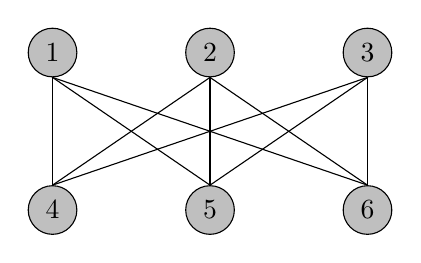
\begin{tikzpicture}
        \node[draw, circle, fill=gray!50] (node1) at (0,2) {1};  
        \node[draw, circle, fill=gray!50] (node2) at (2,2) {2};  
        \node[draw, circle, fill=gray!50] (node3) at (4,2) {3};  
        \node[draw, circle, fill=gray!50] (node4) at (0,0) {4};  
        \node[draw, circle, fill=gray!50] (node5) at (2,0) {5};  
        \node[draw, circle, fill=gray!50] (node6) at (4,0) {6};
        
        \draw (node1.south) -- (node4.north);
        \draw (node1.south) -- (node5.north);
        \draw (node1.south) -- (node6.north);
        \draw (node2.south) -- (node4.north);
        \draw (node2.south) -- (node5.north);
        \draw (node2.south) -- (node6.north);
        \draw (node3.south) -- (node4.north);
        \draw (node3.south) -- (node5.north);
        \draw (node3.south) -- (node6.north);
    \end{tikzpicture} \\
    \vspace{0.5cm}
    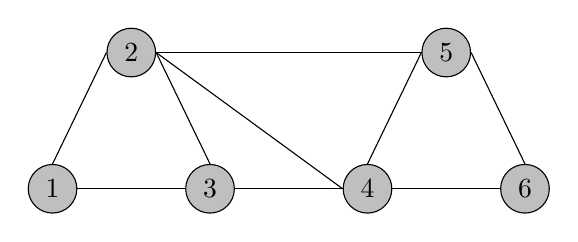
\begin{tikzpicture}
        \node[draw, circle, fill=gray!50] (node1) at (0,0) {1};  
        \node[draw, circle, fill=gray!50] (node2) at (1,1.73) {2};  
        \node[draw, circle, fill=gray!50] (node3) at (2,0) {3};  
        \node[draw, circle, fill=gray!50] (node4) at (4,0) {4};  
        \node[draw, circle, fill=gray!50] (node5) at (5,1.73) {5};  
        \node[draw, circle, fill=gray!50] (node6) at (6,0) {6};
        
        \draw (node1.north) -- (node2.west);
        \draw (node1.east) -- (node3.west);
        \draw (node2.east) -- (node3.north);
        \draw (node4.north) -- (node5.west);
        \draw (node4.east) -- (node6.west);
        \draw (node5.east) -- (node6.north);
        \draw (node2.east) -- (node5.west);
        \draw (node3.east) -- (node4.west);
        \draw (node2.east) -- (node4.west);
    \end{tikzpicture}
\end{center}
\end{document}